\section{Iterations} 

\subsection{\colorbox{cyan}{Project Sprints}}

\begin{table}[!hbt]
\begin{tabular}{|c|c|c|c|}
\hline
\textbf{Sprint \#} & \textbf{Remainder (pts)} & \textbf{Planned (pts)} & \textbf{Completed (pts)} \\ \hline
Sprint 1 & 39 & 12 & 8  \\ \hline
Sprint 2 & 31 & 23 & 21 \\ \hline
Sprint 3 & 10 &    &    \\ \hline
\end{tabular}
\end{table}

\subsection{Sprint 1}

\subsubsection{Plan}
In this sprint we aimed to get a simple working version of Blackjack that runs from a GUI.

\noindent We added 6 (Main, card, deck, hand, player, and game).java that serves as our business logic for our game. Additionally we added a login screen that allows the user to sign in, create an account, or play as a guest. We have also implemented the base for our backend database that stores our users login info.

\subsubsection{Activities (Stories)}

\textbf{Beginning of Sprint 1 (Paired Programming)}

\begin{table}[!hbt]
\begin{tabular}{|l|l|}
\hline
\multicolumn{1}{|c|}{\textbf{Name (pts)}} & \multicolumn{1}{c|}{\textbf{Stories Attempted (pts)}} \\ \hline
Chris, Callie (5)                         & S14(1), S21(1), S26(3)                                \\ \hline
Jenna, Emma (7)                           & S1(2), S2(1), S3(2), S7(2)                            \\ \hline
\end{tabular}
\end{table}



\noindent \textbf{End of Sprint 1 (Paired Programming)}

\begin{table}[!hbt]
\begin{tabular}{|l|l|}
\hline
\multicolumn{1}{|c|}{\textbf{Name (pts)}} & \multicolumn{1}{c|}{\textbf{Stories Accomplished (pts)}} \\ \hline
Chris, Callie (4) & S21(1),  S26(3) \\ \hline
Jenna, Emma (4) & S1(2), S3(2) \\ \hline
\end{tabular}
\end{table}

\pagebreak

\noindent \textbf{Individual Speeds and Cycle times}

\begin{table}[!hbt]
\begin{tabular}{|c|l|c|c|c|}
\hline
\textbf{Name} & \multicolumn{1}{c|}{\textbf{\begin{tabular}[c]{@{}c@{}}Speed\\ (pts)\end{tabular}}} & \textbf{\begin{tabular}[c]{@{}c@{}}Paired \\ Programming\\ ($\div 2$)\end{tabular}} & \textbf{\begin{tabular}[c]{@{}c@{}}Work \\ (hrs)\end{tabular}} & \textbf{\begin{tabular}[c]{@{}c@{}}Cycle\\ (hrs/pts)\end{tabular}} \\ \hline
Chris & 4 & 2 & 35 & 16 \\ \hline
Jenna & 4 & 2 & 40 & 20 \\ \hline
Callie & 4 & 2 & 35 & 17.5 \\ \hline
Emma & 4 & 2 & 29 & 14.5 \\ \hline
\end{tabular}
\end{table}

\subsubsection{Sprint 1 Testing}

Here are the individual testing results for each member:

\begin{table}[!hbt]
\begin{tabular}{|ccc|}
\hline
\multicolumn{1}{|c|}{\textbf{Class}}                                              & \multicolumn{1}{c|}{\textbf{Statement Coverage (\%)}} & \textbf{Branch Coverage (\%)} \\ \hline
\multicolumn{3}{|c|}{\textbf{Chris}}                                                                                                 \\ \hline
\multicolumn{1}{|c|}{Card}                                                      & \multicolumn{1}{c|}{100}           & 100           \\ \hline
\multicolumn{1}{|c|}{Deck}                                                      & \multicolumn{1}{c|}{100}           & 100           \\ \hline
\multicolumn{1}{|c|}{Game}                                                      & \multicolumn{1}{c|}{80}            & 70            \\ \hline
\multicolumn{1}{|c|}{Hand}                                                      & \multicolumn{1}{c|}{97}            & 93            \\ \hline
\multicolumn{1}{|c|}{Player}                                                    & \multicolumn{1}{c|}{100}           & 100           \\ \hline
\multicolumn{1}{|c|}{\textbf{Average}}                                          & \multicolumn{1}{c|}{\textbf{95.4}} & \textbf{92.6} \\ \hline
\multicolumn{3}{|c|}{\textbf{Jenna}}                                                                                                 \\ \hline
\multicolumn{1}{|c|}{\begin{tabular}[c]{@{}c@{}}User\\ Controller\end{tabular}} & \multicolumn{1}{c|}{74}            & 62            \\ \hline
\multicolumn{1}{|c|}{\begin{tabular}[c]{@{}c@{}}Logout\\ Controller\end{tabular}} & \multicolumn{1}{c|}{100}                              & 100                           \\ \hline
\multicolumn{1}{|c|}{\textbf{Average}}                                          & \multicolumn{1}{c|}{\textbf{87}}   & \textbf{81}   \\ \hline
\multicolumn{3}{|c|}{\textbf{Callie}}                                                                                                \\ \hline
\multicolumn{1}{|c|}{\begin{tabular}[c]{@{}c@{}}Game\\ Controller\end{tabular}} & \multicolumn{1}{c|}{91}            & 77            \\ \hline
\multicolumn{1}{|c|}{\textbf{Average}}                                          & \multicolumn{1}{c|}{\textbf{91}}   & \textbf{77}   \\ \hline
\multicolumn{3}{|c|}{\textbf{Emma}}                                                                                                  \\ \hline
\multicolumn{1}{|c|}{App/page}                                                  & \multicolumn{1}{c|}{100}           & 100           \\ \hline
\multicolumn{1}{|c|}{\textbf{Average}}                                          & \multicolumn{1}{c|}{\textbf{100}}  & \textbf{100}  \\ \hline
\end{tabular}
\end{table}

\pagebreak

\subsubsection{(Sprint 1) Retrospective}
We realized that integration between model, view and controller can take much more time than anticipated. Additionally, some of our original point values for our user stories might have been underestimated.

\subsection{\colorbox{cyan}{Sprint 2}}


\subsubsection{\colorbox{cyan}{Plan}}

\noindent Our plan for sprint 2 was to develop the social aspects of the game around our simple functioning version of our game. This included more robust sign in/out, guest user handling, messaging and friend management. We implemented numerous java script and css files that build our GUI using data in our database.

\subsubsection{\colorbox{cyan}{Activities (Stories)}}

\textbf{Beginning of Sprint 2}

\begin{table}[!hbt]
\begin{tabular}{|l|l|}
\hline
\multicolumn{1}{|c|}{\textbf{Name (pts)}} & \multicolumn{1}{c|}{\textbf{Stories Attempted (pts)}} \\ \hline
Chris (8)  & S8(2), S10(2), S12(2), T2(1), T3(1)       \\ \hline
Jenna (7)  & S2(1), S4(1), S5(1), S6(1), S7(2), T1(1) \\ \hline
Callie (6) & S15(1), S22(2), S23(2), T2(1)              \\ \hline
Emma (5)   & S19(2), S20(2), T4(1)               \\ \hline
\end{tabular}
\end{table}

\noindent \textbf{End of Sprint 2}

\begin{table}[!hbt]
\begin{tabular}{|l|l|}
\hline
\multicolumn{1}{|c|}{\textbf{Name (pts)}} & \multicolumn{1}{c|}{\textbf{Stories Accomplished (pts)}} \\ \hline
Chris (9)  & S8(2), S9(2), S10(2), S11(2), T3(1) \\ \hline
Jenna (6)  & S2(1), S4(1), S5(1), S7(2), T1(1)   \\ \hline
Callie (5) & S22(2), S23(2), T2(1)             \\ \hline
Emma (5)   & S19(2), S20(2), T4(1)         \\ \hline
\end{tabular}
\end{table}

\pagebreak

\noindent \textbf{Individual Speeds and Cycle times}

\begin{table}[!hbt]
\begin{tabular}{|c|c|c|c|}
\hline
\textbf{Name} &
  \textbf{\begin{tabular}[c]{@{}c@{}}Speed\\ (pts)\end{tabular}} &
  \textbf{\begin{tabular}[c]{@{}c@{}}Work \\ (hrs)\end{tabular}} &
  \textbf{\begin{tabular}[c]{@{}c@{}}Cycle\\ (hrs/pts)\end{tabular}} \\ \hline
Chris  & 9 & 35 & 3.89  \\ \hline
Jenna  & 6 & 30 & 5     \\ \hline
Callie & 5 & 45 & 9     \\ \hline
Emma   & 5 & 15 & 3     \\ \hline
\end{tabular}
\end{table}

\subsubsection{\colorbox{cyan}{Sprint 2 Testing}}

Here are the individual testing results for each member:

\begin{table}[!hbt]
\begin{tabular}{|ccc|}
\hline
\multicolumn{1}{|c|}{\textbf{Class}} & \multicolumn{1}{c|}{\textbf{Statement Coverage (\%)}} & \textbf{Branch Coverage (\%)} \\ \hline
\multicolumn{3}{|c|}{\textbf{Chris}}                                                          \\ \hline
\multicolumn{1}{|c|}{TableList}          & \multicolumn{1}{c|}{100}           & 100           \\ \hline
\multicolumn{1}{|c|}{TableInfo}          & \multicolumn{1}{c|}{100}           & 100           \\ \hline
\multicolumn{1}{|c|}{JoinTable}          & \multicolumn{1}{c|}{96}            & 92            \\ \hline
\multicolumn{1}{|c|}{CreateTable}        & \multicolumn{1}{c|}{80}            & 62            \\ \hline
\multicolumn{1}{|c|}{{[}tableId{]}/page} & \multicolumn{1}{c|}{100}           & 100           \\ \hline
\multicolumn{1}{|c|}{\textbf{Average}}   & \multicolumn{1}{c|}{\textbf{95.2}} & \textbf{90.8} \\ \hline
\multicolumn{3}{|c|}{\textbf{Jenna}}                                                          \\ \hline
\multicolumn{1}{|c|}{ManageFriends}      & \multicolumn{1}{c|}{100}           & 100           \\ \hline
\multicolumn{1}{|c|}{FriendsList}        & \multicolumn{1}{c|}{85.4}          & 70            \\ \hline
\multicolumn{1}{|c|}{UserList}           & \multicolumn{1}{c|}{92.8}          & 75            \\ \hline
\multicolumn{1}{|c|}{\textbf{Average}}   & \multicolumn{1}{c|}{\textbf{92.7}} & \textbf{81.7} \\ \hline
\multicolumn{3}{|c|}{\textbf{Callie}}                                                         \\ \hline
\multicolumn{1}{|c|}{CardDisplay}        & \multicolumn{1}{c|}{65}            & 75.5          \\ \hline
\multicolumn{1}{|c|}{\textbf{Average}}   & \multicolumn{1}{c|}{\textbf{65}}   & \textbf{75.5} \\ \hline
\multicolumn{3}{|c|}{\textbf{Emma}}                                                           \\ \hline
\multicolumn{1}{|c|}{Context/auth}       & \multicolumn{1}{c|}{89.1}          & 80            \\ \hline
\multicolumn{1}{|c|}{Loading}            & \multicolumn{1}{c|}{100}           & 100           \\ \hline
\multicolumn{1}{|c|}{layout}             & \multicolumn{1}{c|}{88.6}          & 57.1          \\ \hline
\multicolumn{1}{|c|}{Stats}              & \multicolumn{1}{c|}{89.7}          & 80            \\ \hline
\multicolumn{1}{|c|}{Login}              & \multicolumn{1}{c|}{91.6}          & 71.4          \\ \hline
\multicolumn{1}{|c|}{SignUp}             & \multicolumn{1}{c|}{93.2}          & 90            \\ \hline
\multicolumn{1}{|c|}{\textbf{Average}}   & \multicolumn{1}{c|}{\textbf{92}}   & \textbf{79.8} \\ \hline
\end{tabular}
\end{table}


\begin{figure}[!hbt]
    \centering
    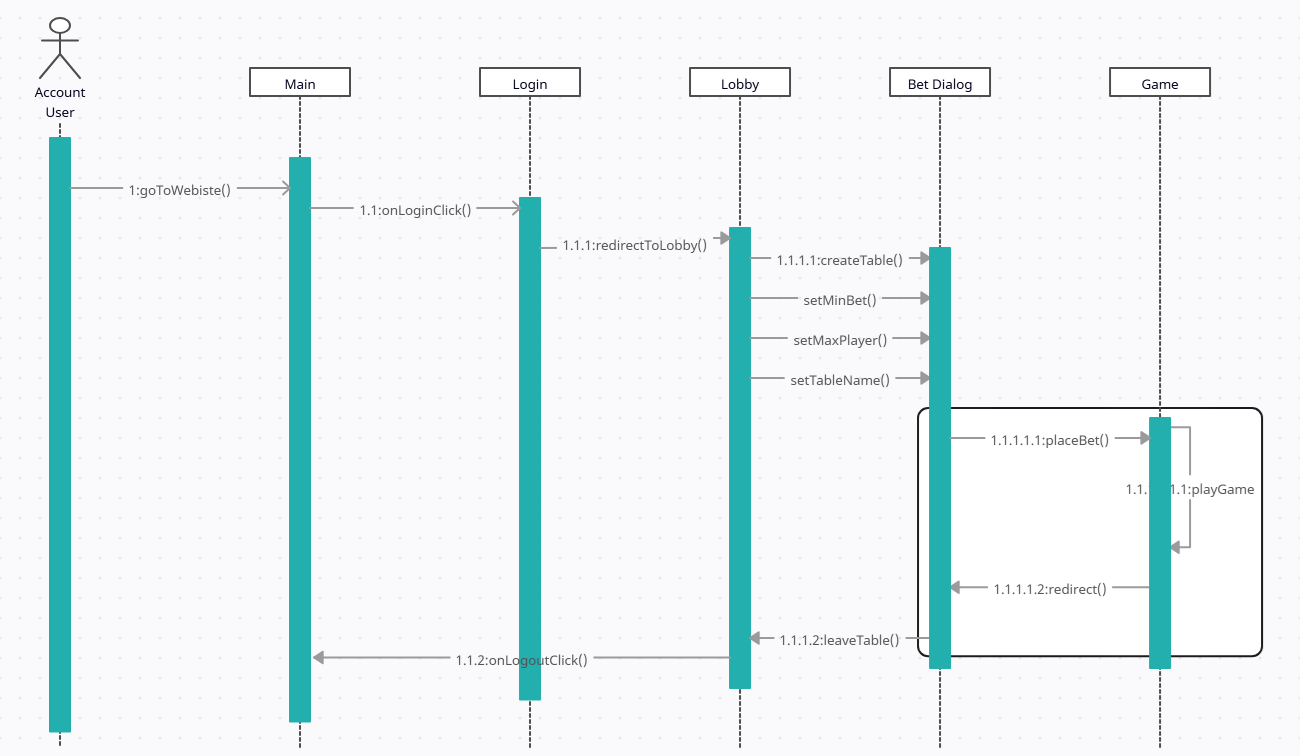
\includegraphics[width=1.0\linewidth]{figures/sequence.png}
    \caption{Sequence Diagram for a user playing the game}
    \label{fig:sequence}
\end{figure}

\subsubsection{\colorbox{cyan}{(Sprint 2) Retrospective}}
In this sprint we realized multiple things including the importance of planning stories. We were fortunate that we planned our stories based on core components of the app. Sprint 1 was focused on the model components of the app allowing us to build all the of the social aspects of the app on top of the existing model components. Additionally, we realized the importance of having the "main" branch be the most current working version of our project. Each member should push to their branch and then move it to main so that everyone else pulls from main rather than pulling from each other. This ensures that main is always up to date and compiles. We also switched our database from MySQL to Firestore/Firebase. This was a good switch as we were having a lot of trouble with MySQL and Firebase was not only easy to use, but thanks to Jenna it was easy to covert to. 


%[[ The requirements analysis identifies \textbf{what} your client wants.
%With each iteration describe the \textbf{how}.
%Include user stories attempted, data structures introduced, and any key design
%decisions.

%Copy this layout for each iteration. ]]


